\documentclass[11pt]{amsart} 
\usepackage{geometry}
\geometry{a4paper}       
\usepackage{graphicx}


\title{Roof Shape}
\author{Sean}

\begin{document}
\maketitle

Roof shape data was taken from the Ethographic Atlas (made available by D-PLACE, see table \ref{roofFreq}). Figure \ref{tree} shows the roof shape for societies speaking Indo-European languages. The trait shows a strong phylogenetic signal (Pagel's $\lambda$ = \input{../results/IndoEuropean_RoofTypes_Lambda.txt}).

% latex table generated in R 3.6.2 by xtable 1.8-4 package
% Thu May 13 13:34:56 2021
\begin{table}[ht]
\centering
\begin{tabular}{rr}
  \hline
 & Frequency \\ 
  \hline
Beehive shaped &  57 \\ 
  Conical & 353 \\ 
  Flat &  95 \\ 
  Four slopes &  88 \\ 
  Hemispherical & 103 \\ 
  One slope &  15 \\ 
  Rounded or semi-cylindrical &  38 \\ 
  Semi-hemispherical &   8 \\ 
  Two slopes & 377 \\ 
   \hline
\end{tabular}
\caption{Frequency of roof shape types} 
\label{roofFreq}
\end{table}


\begin{figure}[h]
\caption{Phylogenetic tree showing roof shape}\label{tree}
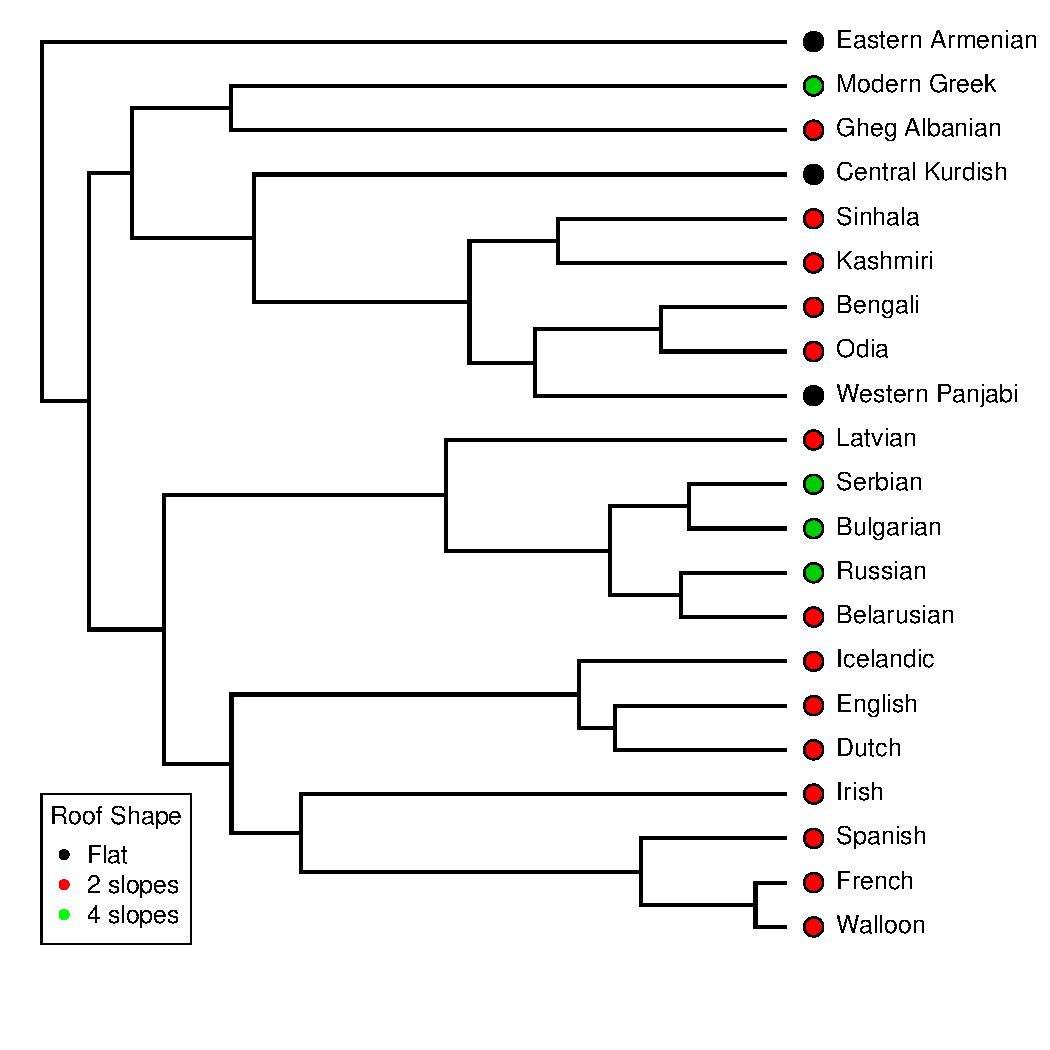
\includegraphics[width=8cm]{../results/IndoEuropean_RoofTypes.pdf}
\end{figure}

\end{document}  